%\documentclass[aspectratio=34]{beamer}
\documentclass{beamer}

% Remove the gratuituous footer
\setbeamertemplate{footline}{}
\setbeamertemplate{navigation symbols}{}
%\renewcommand{\insertnavigation}[1]{}

\usepackage{rotating}
\usepackage{subfigure}
\usepackage{algorithm}
\usepackage{algorithmicx}
\usepackage{algpseudocode}
\usepackage{xcolor}
\usepackage{tabularx}

\usepackage{graphicx}
\DeclareMathOperator{\conv}{conv}
\DeclareMathOperator{\st}{s.t.}
\DeclareMathOperator{\dom}{dom}
\DeclareMathOperator{\im}{im}
\DeclareMathOperator{\Ne}{Ne}
\DeclareMathOperator{\sign}{sign}
\DeclareMathOperator{\Var}{Var}
\DeclareMathOperator{\diag}{diag}
\DeclareMathOperator{\vvec}{vec}


%\usepackage{beamerthemesplit}

% Make footnotes visible. Stolen from http://tex.stackexchange.com/questions/5852/beamer-footnote-text-collides-with-navigation-symbols
\addtobeamertemplate{footnote}{\vspace{-6pt}\advance\hsize-0.5cm}{\vspace{6pt}}
\makeatletter
% Alternative A: footnote rule
\renewcommand*{\footnoterule}{\kern -3pt \hrule \@width 2in \kern 8.6pt}
% Alternative B: no footnote rule
% \renewcommand*{\footnoterule}{\kern 6pt}
\makeatother

\setbeamertemplate{bibliography item}{}
\usepackage[style=authoryear-comp,natbib=true,firstinits,doi=true,isbn=false,url=false,eprint=false,backend=biber]{biblatex}
%\usepackage[sorting=none,firstinits,doi=false,isbn=false,url=false,backend=biber]{biblatex}
\bibliography{ML}
% Don't display series
\AtEveryBibitem{\clearlist{series}}
\AtEveryBibitem{\clearfield{series}}
\DeclareSourcemap{
  \maps[datatype=bibtex]{
    \map{
       \step[fieldset=series, null]
    }
  }
}

\DeclareFieldFormat{titlecase}{\MakeTitleCase{#1}}

% Correct casing for journal titles.
\newrobustcmd{\MakeTitleCase}[1]{%
  \ifthenelse{\ifcurrentfield{booktitle}\OR\ifcurrentfield{booksubtitle}%
    \OR\ifcurrentfield{maintitle}\OR\ifcurrentfield{mainsubtitle}%
    \OR\ifcurrentfield{journaltitle}\OR\ifcurrentfield{journalsubtitle}%
    \OR\ifcurrentfield{issuetitle}\OR\ifcurrentfield{issuesubtitle}%
    \OR\ifentrytype{book}\OR\ifentrytype{mvbook}\OR\ifentrytype{bookinbook}%
    \OR\ifentrytype{booklet}\OR\ifentrytype{suppbook}%
    \OR\ifentrytype{collection}\OR\ifentrytype{mvcollection}%
    \OR\ifentrytype{suppcollection}\OR\ifentrytype{manual}%
    \OR\ifentrytype{periodical}\OR\ifentrytype{suppperiodical}%
    \OR\ifentrytype{proceedings}\OR\ifentrytype{mvproceedings}%
    \OR\ifentrytype{reference}\OR\ifentrytype{mvreference}%
    \OR\ifentrytype{report}\OR\ifentrytype{thesis}}
    {#1}
{\MakeSentenceCase{#1}}}

%%%%%%%%%%%%%%%%%%%%%%%%%%%%%%%%%%%%%%%%%%%%%%%%%%%%%%%%%%%%%%%%%%%%
%% THE ACTUAL DOCUMENT BEGINS
%%%%%%%%%%%%%%%%%%%%%%%%%%%%%%%%%%%%%%%%%%%%%%%%%%%%%%%%%%%%%%%%%%%%

\title{Topic Models for Texts and Images in Representation Space}
\author{Kui Tang and Sameer Lal}
\institute{Columbia University}

\date{29 April 2015}

\begin{document}

\frame{\titlepage}

\begin{frame}
  \frametitle{Outline}
  \begin{enumerate}
    \item Review topic models and multimodal embeddings.
      \begin{enumerate}
        \item Proposed joint model
        \item Actual layer-wise model.
        \item Data
      \end{enumerate}
    \item Image-word alignment model (DeViSE) \citep{Frome13}.
      \begin{enumerate}
        \item Results
        \item Demo
      \end{enumerate}
    \item Mixture of Gaussian topic model (original work).
    \begin{enumerate}
      \item Comparison to baseline LDA
      \item Text training
      \item Text + image training. 
      \item Demo
    \end{enumerate}
    \item Conclusions + future work.
  \end{enumerate}
\end{frame}

\begin{frame}
  \frametitle{Review Topic Models and Multimodal Embeddings.}
\end{frame}

\begin{frame}
  \frametitle{Topic Models}
  {\centering 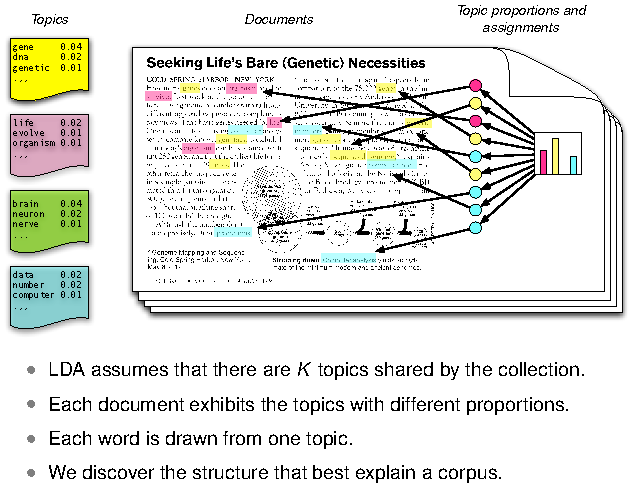
\includegraphics[width=\textwidth]{assets/lda_colors.pdf}}
  {\small \emph{Slide stolen from D. Blei.} \par}
\end{frame}

\begin{frame}
  \frametitle{Latent Variable Models}
  {\centering 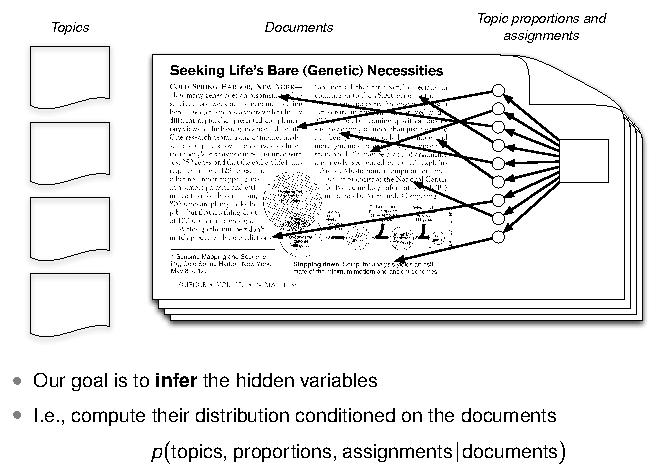
\includegraphics[width=\textwidth]{assets/lda_hidden.pdf}}
  {\small \emph{Slide stolen from D. Blei.} \par}
\end{frame}

\begin{frame}
  \frametitle{Bayesian Networks}
  {\centering 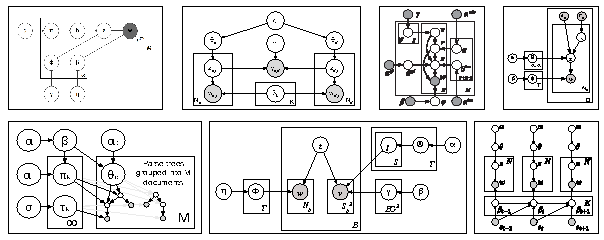
\includegraphics[width=\textwidth]{assets/lda_crazy.pdf}}
  {\small \emph{Slide stolen from D. Blei.} \par}
  \begin{itemize}
  \item Shaded variables are \emph{observed}, other variables are \emph{hidden}.
  \item A model is our hypothesis for how data are generated.
  \item We \emph{condition} on observations to update our hypothesis.
  \end{itemize}
\end{frame}

\begin{frame}
  \frametitle{Multimodal Documents}
  \begin{center}
    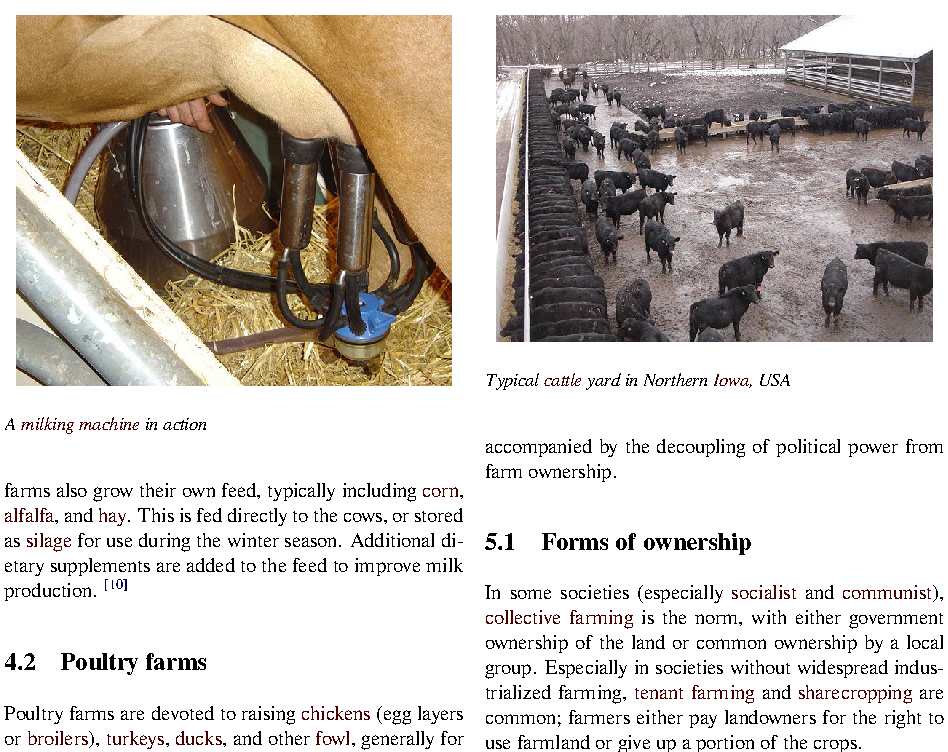
\includegraphics[width=0.75\textwidth]{assets/wiki_farm.pdf}
  \end{center}
             
  \begin{itemize}
  \item \emph{We want to learn a topic model using text and images jointly.}
  \item Images and text complement each other.
  \item Captions aren't the whole story: cows in political contexts.
  \end{itemize}
             
\end{frame}

\begin{frame}
  \frametitle{Proposed joint model (work in progress)}
  \begin{center}
    \includegraphics[width=0.7\textwidth]{gtm_cnn.pdf}
  \end{center}
  {\small
  \begin{itemize}
  \item Topics are (mixtures of) Gaussians.
  \item Words are latent vectors $\lambda_v \in \mathbb{R}^{D_W}$ using Bayesian word2vec.
  \item Images are latent vectors $v_{in} \in \mathbb{R}^{D_I}$ \emph{conditioned} on raw images $x_{di}$. We have $v_{ni} \sim \mathcal{N}(M \text{CNN}_x(x_{ni} ; \Omega), \Sigma)$ with $\Omega$ CNN parameters, $M$ mapping to word vector space, and $\text{CNN}_x$ feature representation output by CNN.
  \end{itemize}
  \par}
\end{frame}

\begin{frame}
  \frametitle{Variational Bayesian EM (eventually)}
  To learn latent variable models, maximize the \emph{marginal likelihood}
  \[
  \max_{\theta}p(\mathbf{x}|\theta)=\int p(\mathbf{x},\mathbf{z}|\theta)p(\mathbf{z}|\theta)d\mathbf{z}
  \]
  This integral is intractable. Approximate instead with the \emph{evidence lower bound (ELBO)}
  \[
  \log p(\mathbf{x}|\theta)\geq E_{q(z|\phi)}\left[\log p(\mathbf{x},\mathbf{z}|\theta)-\log q(\mathbf{z}|\theta)\right]=:{\cal L}(\theta,\phi)
  \]
  {\small where $q(\mathbf{z}|\phi)$ is a simple \emph{variational distribution} which approximates the posterior $p(\mathbf{z}|\mathbf{x},\theta)$. \par}
  \textbf{Variational Bayesian EM:}
  \begin{itemize}
  \item E Step: Update $\phi^{(t+1)}\leftarrow\arg\max_{\phi}\mathcal{L}(\theta^{(t)},\phi)$
  \item M Step: Update $\theta^{(t+1)}\leftarrow\arg\max_{\theta}\mathcal{L}(\theta,\phi^{(t)})$
  \end{itemize}
  {\small 
    E step is variational Bayesian inference \citep{WangC13, Ranganath14}. M step is learning (updating) a CNN with objective
    \par}
  \[ \min_\Omega \sum_\ell L(y_\ell ; \text{CNN}_y(x_\ell ; \Omega)) + \frac{1}{2\sigma^2} \sum_{di} E_{q(v_{di}|\phi^(t))} \left[ (v_{di} - \text{CNN}_x(x_{di} ; \Omega))^2 \right] \]
\end{frame}

\begin{frame}
  \frametitle{Actual layer-wise model}
  \begin{center}
    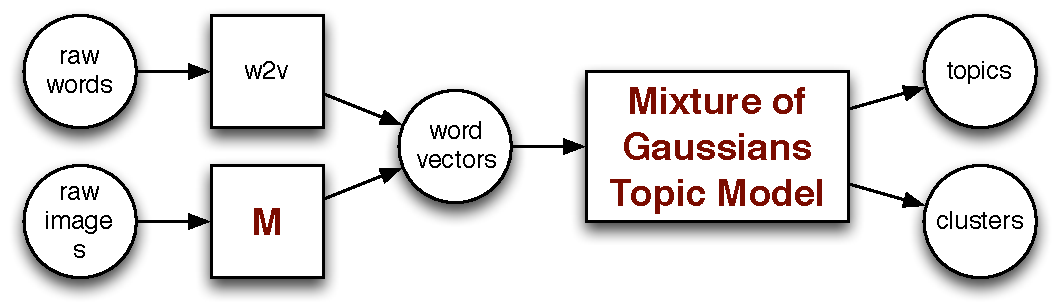
\includegraphics[width=\textwidth]{assets/stagewise_model.pdf}
  \end{center}

  {\small
  \begin{itemize}
    \item Train image-word alignment $M$ and mixture of Gaussian topic model separately.
    \item Pretrained word2vec model on 3 million word/phrase vocabulary, 100 billion word corpus. 
    \item Pretrained Caffe reference network \citep{Jia14}, derived from AlexNet \citep{Krizhevsky12}.
    \item No fine-tuning (for now)
  \end{itemize}
  \par}
\end{frame}

\begin{frame}
  \frametitle{Data}
\end{frame}

\begin{frame}
  \frametitle{Data}
  \begin{itemize}
  \item Imagenet's 1.3 million training images over 1000 classes
  \item Wikipedia pages for each of the 1000 classes
  \item Used Google's Word2Vec pretrained word vectors from the Google News Corpus.
	This corpus had 10 billion words, and generated 3 million word vectors.
  \item Synthetic data
  \end{itemize}
\end{frame}

\begin{frame}
  \frametitle{Extraction of AlexNet Features}
  \begin{center}
    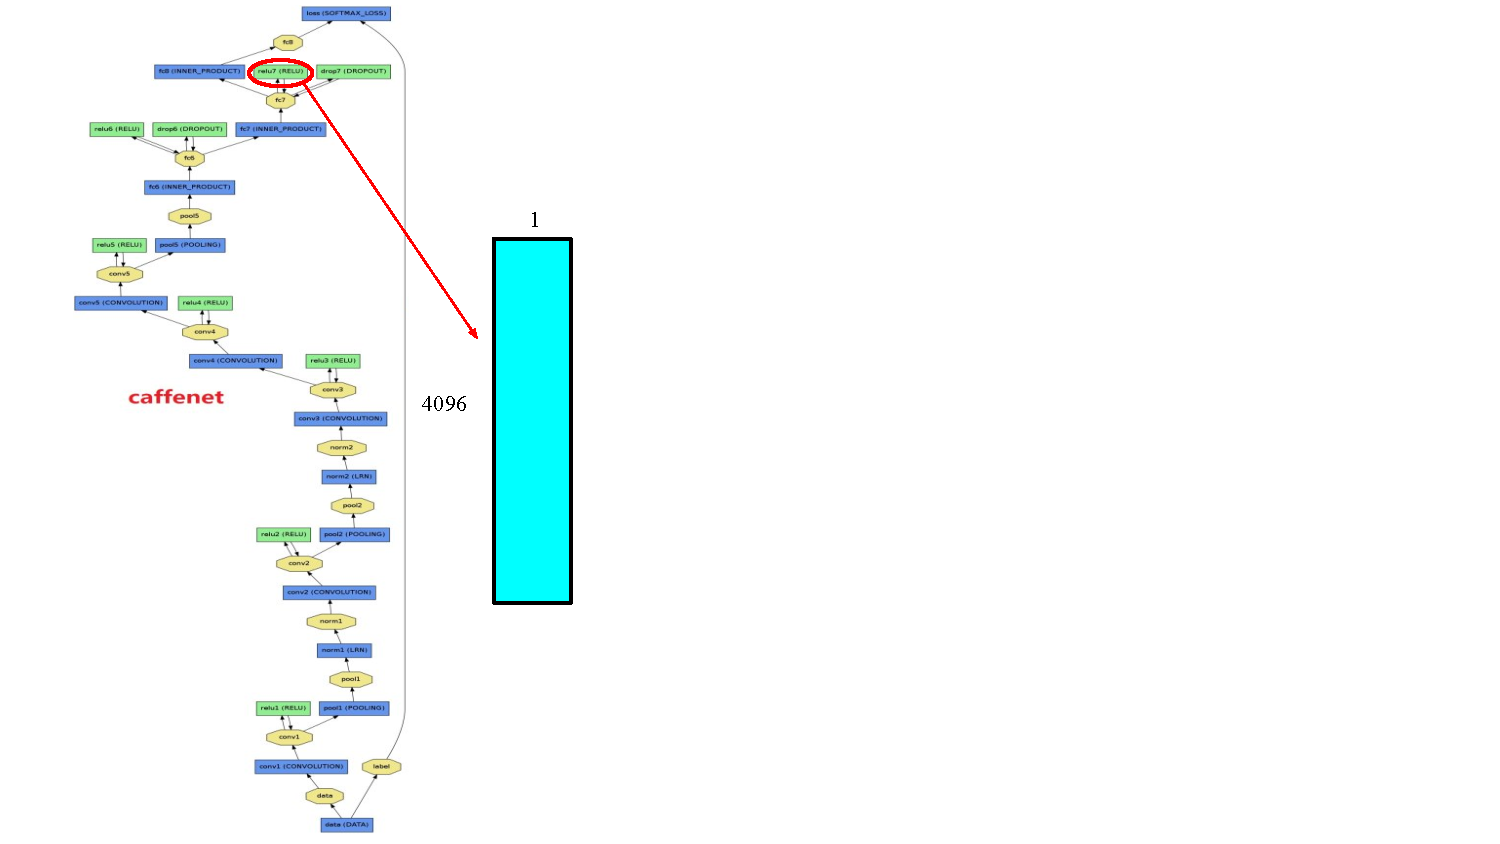
\includegraphics[height=0.9\textheight]{assets/CaffeNetFeatures.pdf}
  \end{center}
%  \begin{itemize}
%    \item Hacked BVLC's Caffe's predefined Caffenet model (found in Model Zoo)
%    \item Extracted layer after the final rectified linear unit
%    \item TODO: EXPLAIN WHY THIS IS IMPORTANT; ADD A DIAGRAM.
%    \item Ran on entire Imagenet
%  \end{itemize}
\end{frame}

\begin{frame}
  \frametitle{Image Vectorization API}
  \begin{center}
    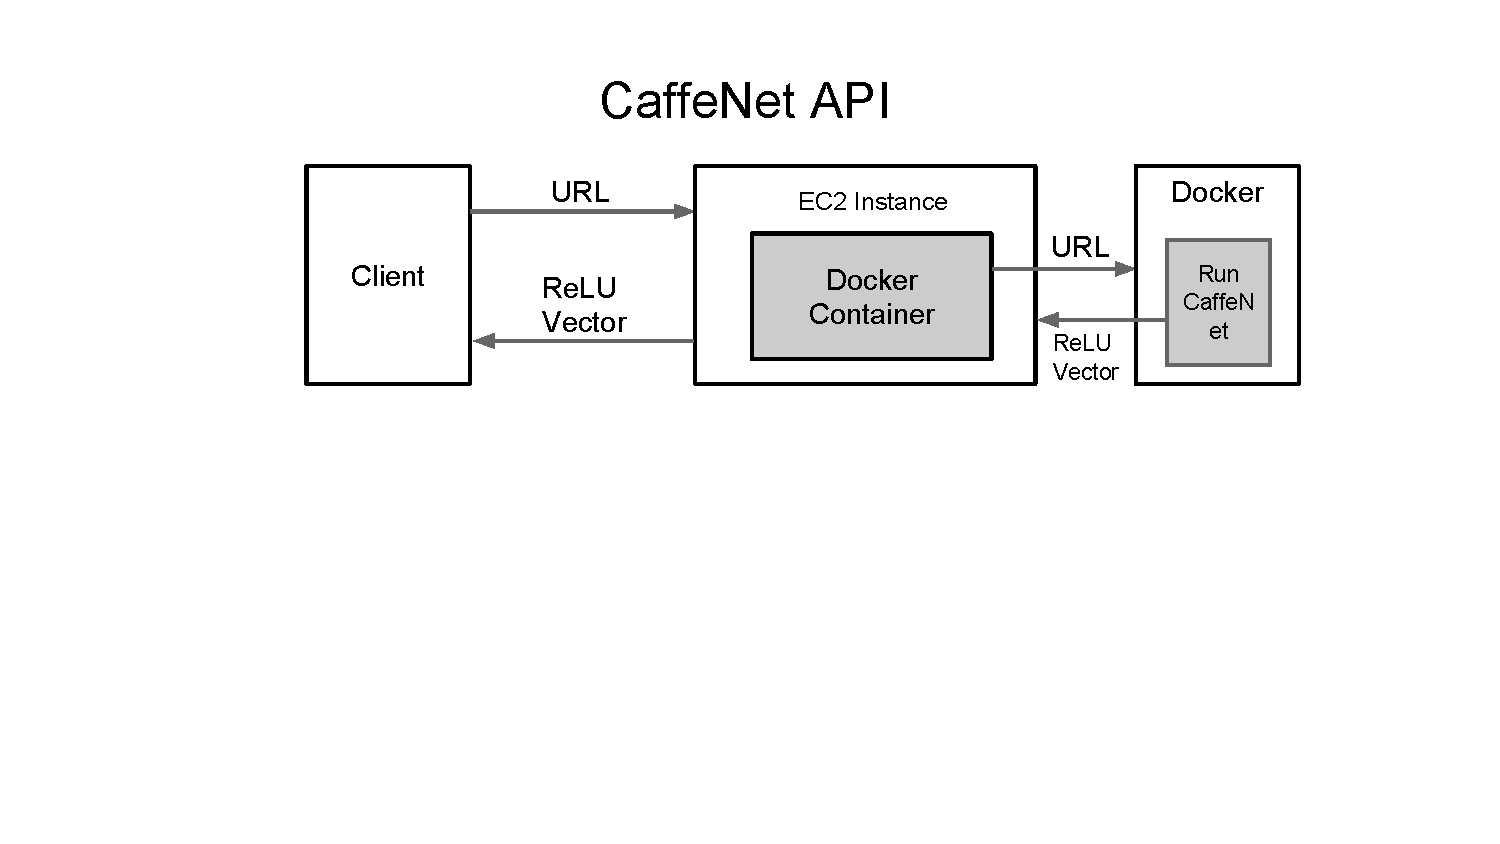
\includegraphics[width=\textwidth]{assets/CaffeNetAPI.pdf}
  \end{center}
  \begin{itemize}
    \item TODO
    \item BTW most groups only did this! [Make sure to remove before presentation.]
  \end{itemize}
\end{frame}

\begin{frame}
  \frametitle{Image-word alignment model ($M$).}
\end{frame}

\begin{frame}
  \frametitle{Transform Raw Images to Word Vectors}
  \begin{center}
    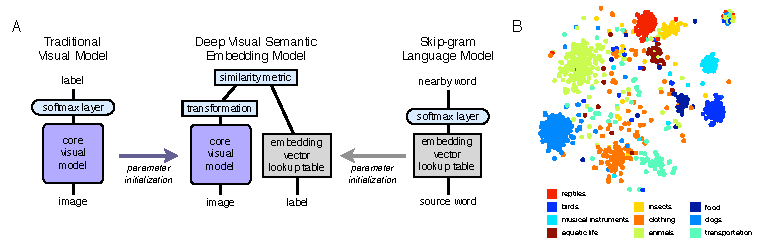
\includegraphics[width=\textwidth]{assets/devise.pdf}
  \end{center}
  \begin{itemize}
    \item Learn $M$ by minimizing a ranking loss: $$\ell(v, y) = \sum_{y' \neq y} \max \left[0, \lambda - w_{y}^\top M v + w_{y'} ^\top M v \right]$$ where $v$ is image vector, $y$ is image label, $w$ is word vector. Sum this term over all $(v, y)$ pairs in labeled data.
    \item Instead of summing all $y' \neq y$, randomly iterate $y'$ and return first example violating the margin.
  \end{itemize}
\end{frame}

\begin{frame}
  \frametitle{Results}
\end{frame}

\begin{frame}
  \frametitle{Demo}
\end{frame}


\begin{frame}
  \frametitle{Comparison to Baseline LDA}
\end{frame}

\begin{frame}
  \frametitle{Baseline LDA Results}
  \begin{itemize}
    \item Extracted and cleaned Wikipedia pages for Imagenet synsets (928 found), stemmed words, kept those in pre-trained word2vec model.
    \item Ran LDA (gensim's implementation)with the following results:
    \begin{itemize}
      \item 20  Topics, Perplexity: \textbf{194.5}
      \item Topic 1: drill, cream, song, album, shower
      \item Topic 2: bird, speci, water, nest, egg
      \item Topic 3: state, school, citi, public, new
      \item Topic 4: car, oper, system, engine, use
      \item Topic 5: speci, male, female, anim, it 
    \end{itemize}
    \item Model 2:
    \begin{itemize}
      \item 100 Topics, Perplexity: 259.0
      \item Topic 1: toaster, ipod, lipstick, mailbox, holstein
      \item Topic 2: speci, plant, fruit, food, seed
      \item Topic 3: pattern, giant, towel, taylor, box
      \item Topic 4: web, toolkit, widget, mod, oar
      \item Topic 5: valley, tractor, pipe, river, hitch
    \end{itemize}
%    \item Model 3:
%    \begin{itemize}
%      \item 500 Topics, Perplexity: >>1,000,000
%      \item Topic 1: platypus, kite, use, speci, male
%      \item Topic 2: bald, speci, use, hummingbird, jellyfish
%      \item Topic 3: goldfish, gila, fish, may, it
%      \item Topic 4: coat, rain, germ, pool, slug
%      \item Topic 5: ostrich, leatherback, water, nest, sea
%    \end{itemize}
  \end{itemize}
\end{frame}

%\begin{frame}
%  \frametitle{DeVISE Re-Implementation Results (Synthetic Data)}
%\end{frame}

\begin{frame}
  \frametitle{Mixture of Gaussians Topic Model}
\end{frame}

\begin{frame}
  \frametitle{Generative Process}
  The model assumes a large dictionary of ``concepts'', which are Gaussian clusters in semantic space. A topic is a mixture of these concepts, and each vector $x_{dn}$ (word or image) is described by a mixture of topics. The generative process is as follows:
  \begin{itemize}
    \item For $k = 1, \ldots, K$ (for each topic):
      \begin{itemize}
        \item Draw $\beta_k \sim \text{Dir}(\alpha)$
        \item Draw $\lambda_k \sim \text{Gamma}(10^{-6}, 10^{-6})$
        \item Draw $\mu_k \sim \mathcal{N}(0, \diag(\tau))$
      \end{itemize}
    \item For $d = 1, \ldots, D$ (for each document):
      \item Draw $\theta_d \sim \text{Dir}(\gamma)$
      \item For $n = 1, \ldots, N_d$ (for each word in document):
      \begin{itemize}
        \item Draw $z_{dn} \sim \text{Mult}(\theta_{dn})$
        \item Draw $c_{dn} \sim \text{Mult}(\beta_{z_{dn}})$
        \item Draw $x_{dn} \sim \mathcal{N}(\mu_{c_{dn}}, \diag(\tau_{c_{dn}})$
      \end{itemize}
  \end{itemize}
\end{frame}

\begin{frame}
  \frametitle{Gaussian LDA Synthetic Problem}
  \begin{center}
    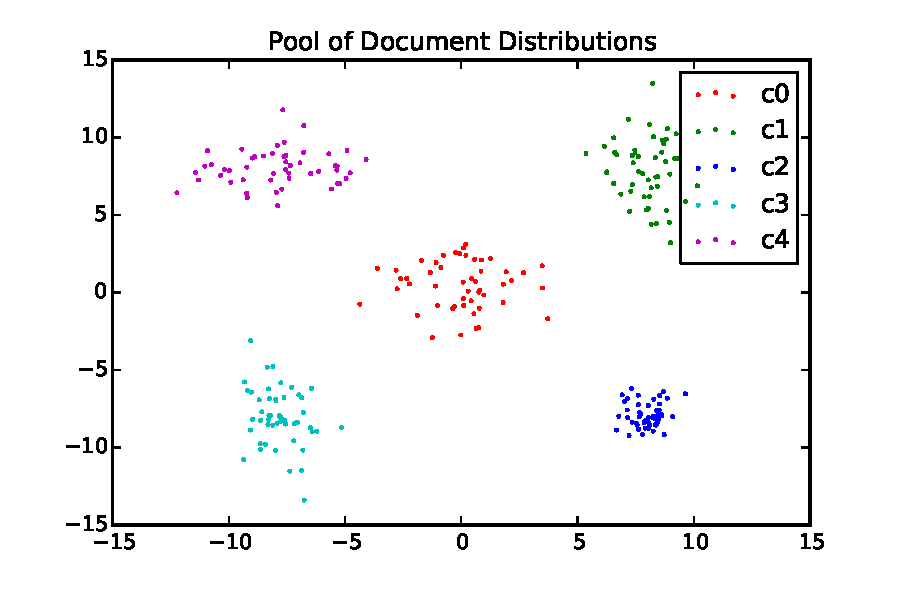
\includegraphics[height=0.2\textheight]{assets/plot.pdf}\\
    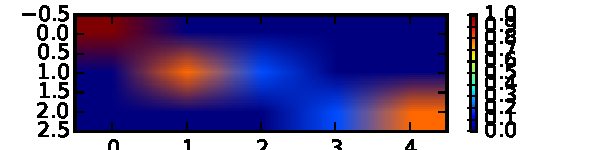
\includegraphics[height=0.2\textheight]{assets/true_topics.pdf}\\
    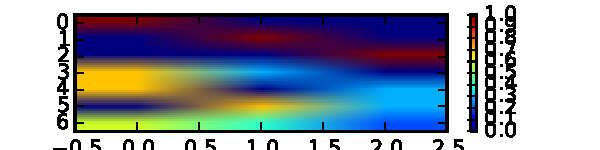
\includegraphics[height=0.2\textheight]{assets/true_document_dictionary.pdf}
  \end{center}
  \begin{itemize}
    {\tiny
    \item Implemented variational message passing \citep{Winn05} and stochastic variational inference using the BayesPy \citep{Luttinen14} package. 
    \item Generate 5 Gaussian clusters (top), 3 topics consisting of mixtures of these clusters (mid) and documents as a mixture of topics.
    }
  \end{itemize}
\end{frame}

\begin{frame}
  \frametitle{Gaussian LDA Synthetic Problem}
  \begin{center}
    \includegraphics[height=0.2\textheight]{assets/remapped_recovered_betas.pdf}\\
    \includegraphics[height=0.2\textheight]{assets/remapped_recovered_thetas.pdf}
  \end{center}
  \begin{itemize}
    \item Recovered essentially the same parameters we used to generate data.
    \item Model is well-specified and approximation algorithm works.
  \end{itemize}
\end{frame}

\begin{frame}
  \frametitle{Mixture of Gaussians Topic Model Results --- Text Only}
\end{frame}

\begin{frame}
  \frametitle{Recovered Topics and Clusters}
  \begin{center}
    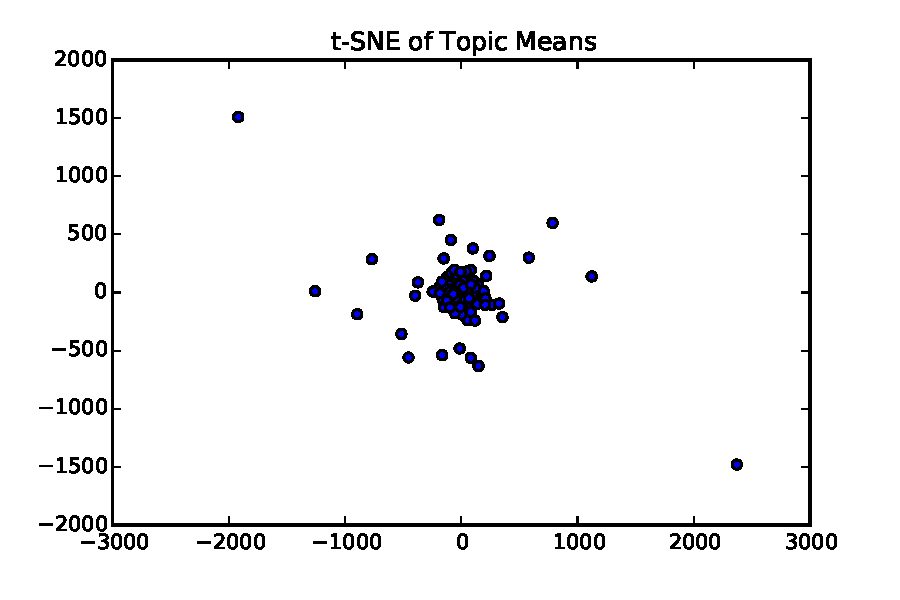
\includegraphics[width=0.5\textwidth]{assets/gtm100_mu_tsne.pdf}
    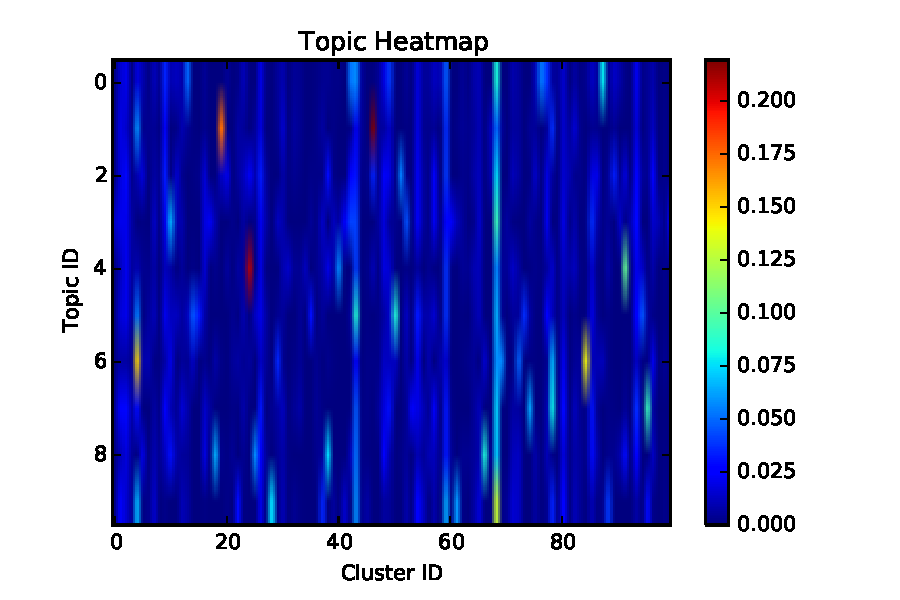
\includegraphics[width=0.5\textwidth]{assets/gtm100_topic_heatmap.pdf}
  \end{center}

  \begin{itemize}
    \item Batch variational inference on 100 docs, 133,866 words.
    \item Selected topics (words from Google News corpus, 3 million word vocabulary.)
      \begin{itemize}
      {\tiny
      \item \textbf{Geography}: east west south north southeast southwest above signs united people regions areas levels states folk properties places sites locations cities
      \item \textbf{Natural resources}: water temperature cold heat temperatures areas regions properties places locations cities towns parts sites natural\_gas electricity gasoline gas fuel electric
      \item \textbf{Music}: game mother folk culture traditions cultural strings vibrato pizzicato trombone instrument Mozart\_concerto orchestra oboe flute cello harpsichord clarinet cellist soprano\_saxophone 
      }
    \end{itemize}
  \end{itemize}
\end{frame}

\begin{frame}
  \frametitle{Example topic and cluster breakdown 1/2}
  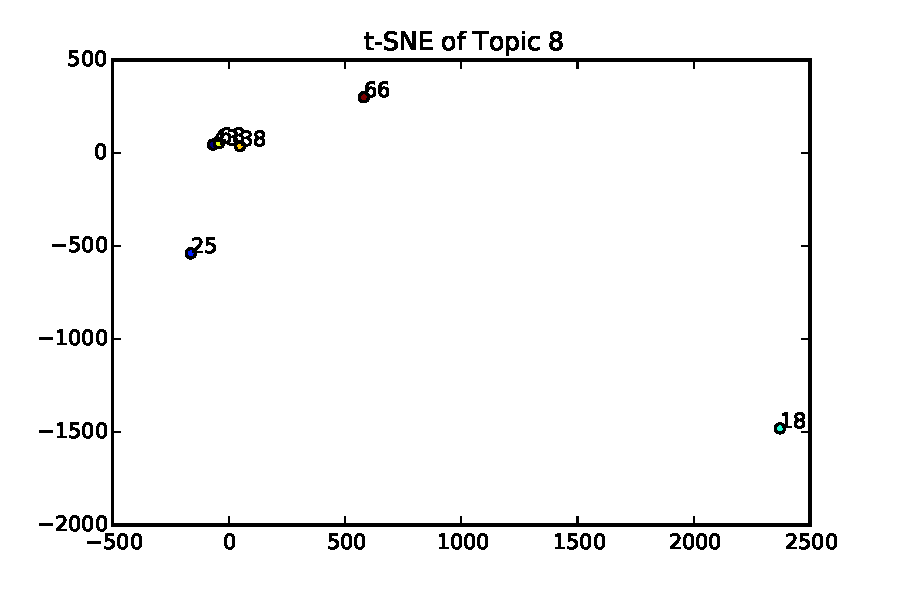
\includegraphics[width=0.5\textwidth]{assets/gtm100_topic8_tsne.pdf}
  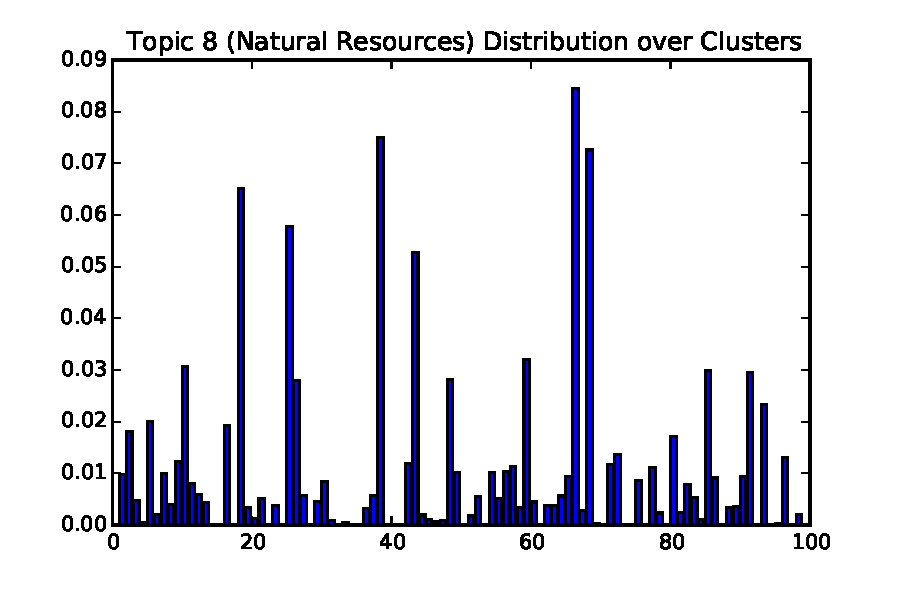
\includegraphics[width=0.5\textwidth]{assets/gtm100_topic8_probs.pdf}

  \begin{tabularx}{\textwidth}{|c|X|}
\hline 
{\tiny{}Cluster} & {\tiny{}Words}\tabularnewline
\hline 
{\tiny{}18} & {\tiny{}\textbf{[Saltwater]} shoreline ocean coastline nearshore\_reefs sandy\_shorelines
coastal\_waters shallow\_reefs tidal\_creek shallow\_waters mud\_flats
sea tidal\_inlet pier\_pilings underwater reef shoreward abyssal\_plain
inter\_tidal shifting\_sandbars sandy\_bottomed }\tabularnewline
\hline 
{\tiny{}25} & {\tiny{}\textbf{[Freshwater]} water ice surface green porpoise\_vaults surficial\_aquifer
rainwater Floridan\_aquifer radar\_deflectors wa\_ter absorbs\_carbon\_dioxide
bermed absorbs\_sunlight bugs\_wiggling Mosquitoes\_breed overflowing\_septic\_tanks
mild\_dishwashing\_liquid reverse\_osmosis\_filtration hyper\_saline
secondary\_clarifier }\tabularnewline
\hline 
  \end{tabularx}

\end{frame}

\begin{frame}
  \frametitle{Example topic and cluster breakdown 1/2}

\begin{tabularx}{\textwidth}{|c|X|}
\hline 
{\tiny{}Cluster} & {\tiny{}Highest Probability Words}\tabularnewline
\hline 
{\tiny{}38} & {\tiny{}\textbf{[Chemicals]} hydrous calcium\_oxide cyclohexane inorganic\_salts calcium\_sulphate
fluorocarbons Sodium\_cyanide silicate\_rocks Nitric\_acid chemically\_reactive
calcium\_carbonates magnesium\_silicate outgas raffinate potassium\_salts
bacterial\_decomposition methane trihalomethanes\_THMs element\_boron
Sulphur\_dioxide }\tabularnewline
\hline 
{\tiny{}66} & {\tiny{}\textbf{[Volcanoes]} coral reefs reef corals coral\_reefs ocean volcanoes sea coral\_reef
volcanic islands lava volcano oceans undersea\_volcanoes oceanic ocean\_basins
lava\_flows eruptions Kilauea\_Volcano}\tabularnewline
\hline 
\end{tabularx}
  
\end{frame}

\begin{frame}
  \frametitle{Properties of Mixture of Gaussian LDA Model}
  \begin{itemize}
    \item Captures both local (word2vec neighborhoods, context) semantic and syntactic similarity, as well as broader topical similarity.
    \item Mixture of Gaussian crucial: components of topic can be \emph{far} in semantic space. Existing global semantic models, e.g. paragraph vectors \citep{Le14q} still require locality in semantic space.
    \item Semantic space representation permits \emph{explaining} topics using a much larger corpus than the training corpus.
    \begin{itemize}
      \item Generalize across corpora.
      \item Get good qualitative results even with small data.
    \end{itemize}
        
  \end{itemize}

\end{frame}

\begin{frame}
  \frametitle{Mixture of Gaussians Topic Model Results --- Text + Images}
\end{frame}

\begin{frame}
  \frametitle{Demo}
\end{frame}

\begin{frame}
  \frametitle{Conclusions + Future Work}
  \begin{itemize}
    \item We have shown a proof-of-concept of a multimodal topic model in representation space:
    \begin{itemize}
      \item Reimplemented DeViSE in CUDA; wrapped into a fast test-time API.
      \item Derived and fit \emph{mixture of Gaussian topic models} (MoGTA), a novel model that can be fit with standard techniques with intriguing properties on pre-trained word vectors.
      \item Demonstrated multimodal inference, modeling vectors for words and images simultaneously.
    \end{itemize}
    \item We have much work to do to make this a proper probabilistic model:
    \begin{itemize}
      \item Improve Bayeisan word2vec to be competitive with non-Bayesian versions.
      \item Join Bayesian word2vec with MoGTA to form one joint model.
      \item Fine-tune image vector updates (variational Bayesian EM).
    \end{itemize}
  \end{itemize}
\end{frame}

\begin{frame}
  \frametitle{Mixture of Gaussians Topic Model --- Text + Images}
\end{frame}

\begin{frame}
  \frametitle{Thank You}
  \begin{itemize}
  \item Questions?
  \end{itemize}
\end{frame}

\section{References}
\begin{frame}[t,allowframebreaks]{}
\frametitle{References}
{\small
\printbibliography
\par}
\end{frame}

\end{document}

